\subsection*{题目背景}

西西艾弗岛景色优美,游人如织。
但是,由于和外界的交通只能靠渡船,交通的不便严重制约了岛上旅游业的发展。
西西艾弗岛管委会经过努力,争取到了一笔投资,建设了一个通用航空机场。
在三年紧锣密鼓的主体建设后,西西艾弗岛通用航空机场终于开始进行航站楼内部软硬件系统的安装和调试工程了。
小 C 是机场运营公司信息部的研发工程师,最近,信息部门的一项重要任务是,研发登机牌自助打印系统。
如图所示的是设计部门根据国际民航组织的行业标准设计的登机牌样张。

\begin{figure}[H]
    \centering
    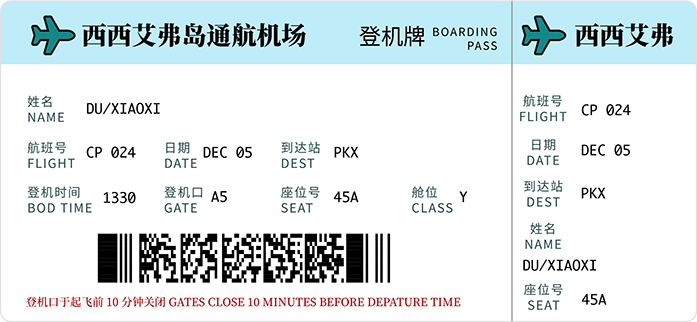
\includegraphics[width=0.95\textwidth]{image/24/3-p-1.png}
\end{figure}

登机牌上最重要的部分就是最下方的机读条形码了。小 C 承担了生成机读条形码算法的开发工作。从被编码的数据到条形码,中间有好多步骤要走。小 C 请你来帮忙,让你帮忙处理一下数据编码的问题。

\subsection*{题目描述}

登机牌上的条形码,是 PDF417 码。PDF417 码的结构如下图所示。

\begin{figure}[H]
    \centering
    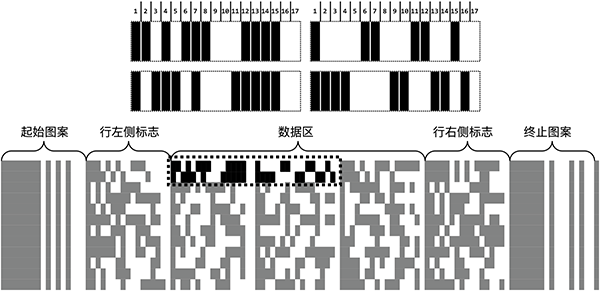
\includegraphics[width=0.95\textwidth]{image/24/3-p-2.png}
\end{figure}

PDF417 码组成的基本元素是码元(Module),所有的码元都是等大的矩形,填充有黑色或白色。码元先组成行,若干行堆叠组成整个 PDF417 码。每一行中,每 17 个码元表示一个{\heiti{码字}}(Code word)。码字是 PDF417 编码中的最小数据单位。每个码字图案中,有交替排列的四个黑色矩形和四个白色矩形,这便是 “417” 的由来。每行开始和结尾有固定的起始和中止图案。与他们相邻的是行左侧和右侧标志,表示行号、行内码字个数等信息。中间的是有效数据区。编码的步骤是:先按照编码规则,将被编码的数据转换为码字;接着根据选定 PDF417 码的宽度(即每行码字的数目)以及冗余程度计算校验码字;最后将码字按规则转换为对应的图案,并按照从左至右,从上至下的的顺序填入有效数据区,并与起始终止图案和行左右标志拼合,形成完整的 PDF417 码。

每个码字是一个 0 至 928 之间的数字,每个码字可以编码两个输入字符。对于输入的被编码的数据,按照下表进行编码。编码器共有三种模式:大写字母模式、小写字母模式和数字模式。在编码开始时,编码器处于大写字母模式。编码器处于某种模式时,仅能编码对应类型的字符,如果需要编码其它类型的字符,需要通过特殊值切换到对应模式下。要进行模式切换,可以有多种切换方法。例如,要从大写模式切入小写模式,可以直接用 27 切入,也可以先用 28 切入数字模式后立刻再用 27 切入小写模式。你需要选择最短的方式进行切换,因此只有前一种方法是正确的。需要注意的是,从小写模式不能直接切入大写模式,必须要经过数字模式过渡。

\begin{table}[H]
\centering
\begin{tabular}{cccc}
    \toprule
    值 & 大写模式 & 小写模式 & 数字模式 \\
    \midrule
    0 & A & a & 0 \\
    1 & B & b & 1 \\
    2 & C & c & 2 \\
    3 & D & d & 3 \\
    4 & E & e & 4 \\
    5 & F & f & 5 \\
    6 & G & g & 6 \\
    7 & H & h & 7 \\
    8 & I & i & 8 \\
    9 & J & j & 9 \\
    10 & K & k &  \\
    11 & L & l &  \\
    12 & M & m &  \\
    13 & N & n &  \\
    14 & O & o &  \\
    15 & P & p &  \\
    16 & Q & q &  \\
    17 & R & r &  \\
    18 & S & s &  \\
    19 & T & t &  \\
    20 & U & u &  \\
    21 & V & v &  \\
    22 & W & w &  \\
    23 & X & x &  \\
    24 & Y & y &  \\
    25 & Z & z &  \\
    27 & 小写 &   & 小写 \\
    28 & 数字 & 数字 & 大写 \\
    29 & 填充 & 填充 & 填充 \\
    \bottomrule
\end{tabular}
\end{table}

按照这个方法可以得到一系列的不超过 30 的数字。
如果有奇数个这样的数字,则在最后补充一个 29,使之成为偶数个。
将它们两两成组,假设 $H$ 和 $L$ 是一组中连续出现的两个数字,那么可以得到一个码字是:

\begin{equation*}
    30 \times H + L
\end{equation*}

例如,要编码 “HE1lo”,首先先根据字母表,产生数字序列:

\begin{lstlisting}
    H E    1    l  o
    7 4 28 1 27 11 14
\end{lstlisting}

由于只有奇数个数字,需要在末尾补充 29,然后将它们两两成组:

\begin{lstlisting}
    (7, 4), (28, 1), (27, 11), (14, 29)
\end{lstlisting}

最后计算码字,例如:$30\times 7+4=214$,以此类推,可以得到码字为:

\begin{lstlisting}
    214, 841, 821, 449
\end{lstlisting}

接下来要计算校验码。
校验码字的数目,由校验级别确定。
假设校验级别为 $s(0\le s\le 8)$,则校验码字的数目为 $k=2^{s+1}$。
特别地,如果指定了 $s=-1$,则表示不需要计算校验码字。
要计算校验码字,首先要确定数据码字。数据码字由以下数据按顺序拼接而成(如图所示):

\begin{figure}[H]
    \centering
    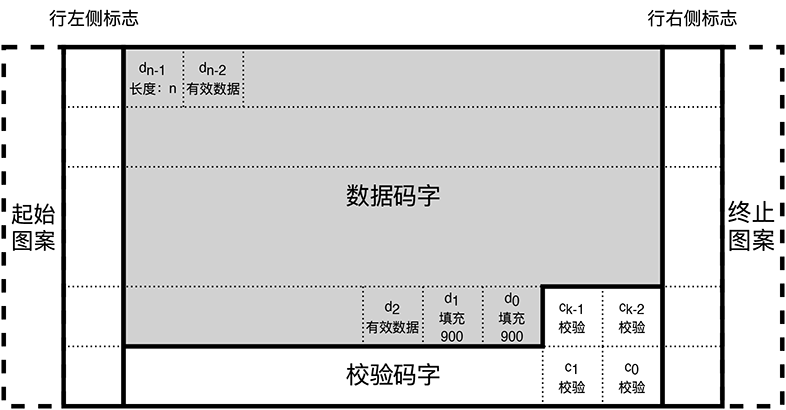
\includegraphics[width=0.95\textwidth]{image/24/3-p-3.png}
\end{figure}

\begin{itemize}
    \item 一个长度码字,表示全部数据码字的个数 $n$,包括该长度码字、有效数据码字、填充码字;
    \item 若干有效数据码字,是此前计算的码字序列;
    \item 零个或多个由重复的 900 组成的填充码字,使得包括校验码字在内的码字总数恰能被有效数据区的行宽度整除。
\end{itemize}

设全部数据码字依次为 $d_{n-1},d_{n-2},\cdots,d_0$
;校验码字依次为 $c_{k-1},c_{k-2},\cdots,c_0$
。那么校验码字按照如下方式计算:

取 $k$ 次多项式 $g(x)=(x-3)(x-3^2)\cdots(x-3^k)$
, $(n-1)$ 次多项式 $d(x)=d_{n-1}x^{n-1}+d_{n-2}x^{n-2}+\cdots+d_1x+d_0$
,找到多项式 $q(x)$ 和不超过 $k-1$ 次的多项式 $r(x)$,使得

\begin{equation*}
    x^kd(x)\equiv q(x)g(x)-r(x)
\end{equation*}

那么多项式 $r(x)$ 中 $x$ 的 $i$ 次项系数对 929 取模后(取正值)的数字即为校验码字 $c_i$
。

例如,如果要将 HE1lo 编码为 PDF417 条码,且有效数据区的行宽是 4 码字(即 68 码元),校验级别为 0。此时校验码字有两个。根据此前的编码结果,有效数据码字有 4 个。再加上一个长度码字,共有 7 个码字。因此需要补充一个填充码字,使包括校验码字在内的总码字数能够被 4 整除。这样,用于计算校验码字的数据码字有 6 个,分别是:

\begin{lstlisting}
    6, 214, 841, 821, 449, 900
\end{lstlisting}

因此有 $g(x)=x^2-12x+27$
,$d(x)=6x^5+214x^4+841x^3+821x^2+449x+900$
,不难得到 $r(x)=-32902164x+98246277$,因此相应可以计算出 $c_1=299\equiv -32902164\mod 929$
,$c_0=811\equiv 98246277\mod 929$
。这样,全部码字序列即为:

\begin{lstlisting}
    6, 214, 841, 821, 449, 900, 229, 811
\end{lstlisting}

在本题中,你需要帮助小 C 完成的任务是,给定被编码的数据,计算出需要填入有效数据区的码字序列。被处理的数据中只含有大写字母、小写字母和数字。

\subsection*{输入格式}

从标准输入读入数据。

输入的第一行包含两个用空格分隔的整数 $w$、$s$,分别表示有效数据区每行能容纳的码字数和校验级别。
保证 $0<w<929$,$-1\le s\le 8$。特别地,当 $s=-1$ 时,表示不需要计算校验码字。

输入的第二行是一个非空字符串,仅包含大小写字母和数字,长度保证编码后全部数据码字的个数少于 929。

\subsection*{输出格式}

输出到标准输出。

输出若干行,每行一个数字,表示编码后的全部码字序列。

\subsection*{样例}

输入\#1:

\begin{lstlisting}
5 -1
HELLO
\end{lstlisting}

输出\#1:

\begin{lstlisting}
5
214
341
449
900
\end{lstlisting}

解释\#1:

要求编码数据是 HELLO,首先查表将其对应成数字。
注意,由于编码器在开始时就处于大写字母模式,因此不需要额外的模式切换。
因此对应成的数字为:7, 4, 11, 11, 14。
由于只有奇数个数字,因此补充 29,形成序列 7, 4, 11, 11, 14, 29。
然后两两成组计算码字:$7\times 30+4=214$,以此类推,得到 214, 341, 449。
本输入不要求产生校验码,且有效数据区的宽度是 5 码字。
目前有效数据的码字是 3 个,加上开头要添加的长度码字,共有 4 个码字。
因此,需要补充一个填充码字,使得总码字数达到 5 个,充满一行。
注意,长度码字中的长度数据包括所有数据码字,因此长度码字是 5 而不是 4。
最终可以得到码字序列 5, 214, 341, 449, 900。

输入\#2:

\begin{lstlisting}
4 0
HE1lo
\end{lstlisting}

输出\#2:

\begin{lstlisting}
6
214
841
821
449
900
229
811
\end{lstlisting}

解释\#2:

本组数据即为此前用于说明编码过程的示例。

\subsection*{子任务}

对于 $20$\% 的数据,有 $s=-1$,且输入字符串中仅含有大写字母或小写字母;

对于 $40$\% 的数据,有 $s=-1$;

对于 $80$\% 的数据,有 $s\le 2$;

对于 $100$\% 的数据,满足全部对于输入的要求。